
\setcounter{chapter}{-1}
%\part{Logic}
%<*logic.Title>
\chapter{Introductory Challenges}\label{logicProblems}
%</logic.Title>
%</logic.intro>

\setcounter{section}{-1}
\section{Mathematical Outcome}

The mathematical process is deeper than simply arriving at the correct answer. The goal of this chapter is to introduce the students and the instructor to the format of the text. The authors' hope is that the activities provided throughout the text will foster an interactive and cooperative classroom environment. This chapter is a set of logic problems which require little or no prerequisite knowledge and establish a foundation of thinking which will be used in activities throughout the text. 

You will find that the students will begin developing the basic problem solving skills throughout this chapters activities. They will encounter such questioning as; ``Is this the optimal answer?'' ``Can we show there is not a better way?''  ``Can we explain why our technique will solve the problem?'' etc. In answering these questions students are engaged in the mathematical method of developing reasoning through concrete examples.

To further this extension from the concrete to the abstract we begin asking students to change the variable of the problem to see if the previous solution technique continues to apply. In some cases a technique can be developed which will work for all possible arrangements of which it is natural to ask ``how do we know the method will work for all possibilities?'' However, the students are also exposed to solution methods which are not valid when a variable is changed. The contrast in the problems will hopefully develop the necessary curiosity which initiates the investigation process.

As a framework for the entire course, Polya's four step method for problem solving should be introduced, emphasized, and reemphasized throughout. Reference to these steps will be made from time to time within the instructor's notes, but they should be kept in the forefront of students' minds whether the prompts are there or not.

Polya's Problem Solving Method
\begin{enumerate}
\item Understand the problem (This may include reading the question several times, asking "what if" questions, tinkering with parts of the question, and so on.)
\item Devise a plan (Though this is often a completely separate step from understanding the problem, the tinkering used to understand may lead to an idea for a plan of action.)
\item Carry out the plan (When the plan can be completed, great! However, one may find they are unable to complete their plan of action due to its difficulty or faultiness. It is at this point, the method becomes iterative. The problem solver will need to revisit understand the problem or devising a plan to refine their approach.)
\item Review (Even when the plan can be carried out successfully, a review of the result is needed. Do the results answer the question asked? What evidence is there that the results are correct? Is that answer actually correct? If not, here is another place where the method becomes iterative. The problem solver will have to revisit one of the first three steps depending on the flaw identified.)
\end{enumerate}
It is important to emphasize that a natural part of problem solving is temporary failure. Noticing that there is a flaw in the solution to a problem (during the review) is a critical step in solving difficult problems. It should not be expected that anyone will devise correct, complete answers on their first try, and that this should not be considered failure. It is a temporary setback that should launch the problem solver down a new path. One only fails when one gives up trying new ideas.


\newpage

\section{Activity: Manager's Schedule}

\noindent Let's assume you are the manager for some business. This could be anything like an advertising firm, a theater production, or IT department. You have 9 projects that must be completed before your team can go on break. You predict that each project will take a day to complete and have assigned the expects needed for each project in the table below. No person can work on two projects in a single day but must be present the entire day the project is being worked on. (Maybe they are in different locations, national safety procedure require this, etc.)  Unfortunately you have to stay until all projects are completed, so you really want to create a schedule that allows yourself to go on break ASAP!

\begin{tabular} {| l | l|}
\hline
Project Number& Employees assigned\\
\hline
\hline
1 & Anna, Beth, Chris, Doug \\
\hline
2 & Eve, Chris\\
\hline
3 & Doug,Eve,Fran,Ian\\
\hline
4 & Anna, Eve, Fran\\
\hline
5 & Beth, Chris, Fran, Greg, Hugh\\
\hline
6 & Anna, Hugh, Ian\\
\hline
7 & Doug, Greg, Hugh\\
\hline
8 & Beth, Greg\\
\hline
9 & Ian \\
\hline
\end{tabular}

\begin{enumerate}

\item \label{firstschedule} Give a first attempt at making a good project schedule. Don't worry about making it on the fewest number of days yet.
\par\Instr{ We are starting to develop Polya's 4 steps in problem solving without calling them by name. We also want to establish a culture of working together and getting something on paper as soon as we start working. Even if students don't have the full or correct answer, they should right down their first attempt to get something to discuss. (I like to refer to these as a ``productive fail'' - you have a product that may have failed your overall goal, but your are progressing in the problem solving process!)}
 \wbvfill
 
\item Double check the schedule you made for Question \ref{firstschedule} to make sure no person is required to work on two projects in the same day. Describe or illustrate how you know your schedule has met that criteria.
\par\Instr{Here we are having the explore the features of the problem to ensure they accurately understand and can explain how a solution they created meets the problem constraints. Seemingly the easiest way for them to check is to write each project for a day and under the project list the employees assigned to that project. They may want to list all the ``inactive'' members as well just to ensure they have accounted for all 9 employees each day. 

\

We suggest at some point when most groups have finished this question to have groups share their schedules with the whole class and discuss their organization process. }
 \wbvfill
 
 \wbnewpage
  
\item Create a way to organize the interactions between the project members. How will you use this information to make a project schedule with the fewest number of days?
\par\Instr{After making a schedule and seeing other groups, students should see that they cannot just simply trial and error this process. So we are now asking the students to re-examine the information from the problem and start to devise a plan by identifying all key variables, data, and or structure of the problem.}
 \wbvfill
 

\item \label{trivialmin}Can you easily identify a minimum number of days you will need your team to work? What is your reasoning you cannot finish any sooner?
\par\Instr{Here we are asking student to stop and identify some easy constraints. Often student get to involved in the problem and don't make simple observations or estimates for their desired solution. The simplest observation here is that every employee has been assigned to three projects, so no schedule could ever exist on fewer than three days. There is also an argument, using graph theory, that no schedule on three days can exist, but that is not an observation we expect at this point. }
 \wbvfill
 
\item Now create a project schedule That uses that uses the fewest number of days
\par\Instr{ This is where we are asking them to carry out their plan. Usually this is the longest period of time in the problem solving process. Notice they are already five questions into the problem before they need to really find the desired solution. This is intentional in giving the students early success and developing a sense that the problem is achievable even if it is hard.

\

There are a lot of schedules that can be made, but one on four days is the optimal solution. One tip for finding this solution is to look at project 5, which cannot be scheduled on the same day as projects 2, 3, 4, 6, or 7. Now just focus on scheduling these other five projects on two days and you will easily find a contradiction. 

\

This can be modeled with graph theory in a process called graph coloring, but at this point in the class we are simply exploring how to search for features that will help problem solve.}
 \wbvfill
 
\item Does your schedule get you on break as early as your answer from Question \ref{trivialmin}? If not, explain why there is no schedule that finishes faster or make a better schedule.
\par\Instr{This is the final step for polya's process, where we ask students to reflect on their solution. Assuming the student answers three days for Question \ref{trivialmin}, they will never achieve this under the constraints of the problem. In the previous explanation we have given you one reason that four days is the optimal answer, but it is not the only reason. 

Having students articulate aspects of their solution and the problem constraints is crucial in understanding the problem and being able to repeat or abstract the process. If time allows, we highly encourage groups sharing their answers to this questions for the whole class to benefit from the knowledge gained.}
\end{enumerate}
 \wbvfill
\newpage

\subsection{Exit Slip: The Manager's Process}

\noindent It is likely you will need to do this again with next year's schedule, but there may be a different number of projects or employees at that time. To help you remember what you learned for next year or possibly pass this along to the next manager, write down the process of find a optimal schedule making sure to highlight at least three things you learned are important about the process.

\par\Instr{We aren't looking for much of a specific answer with this exit slip. This is intended for them to get use to reflecting on the process with the intent to abstract the mathematics they learned. We will develop this throughout the course via exit slips, in hopes this becomes a natural process of problem solving.}

\newpage

\section{Activity: Making \$20}

\begin{center}How many different ways can you have \$20 in US bills?
\end{center}

\noindent Sometimes a simple question can have many layers, so we first must unpack and organize our thoughts before answering! We will use Polya's 4-step problem solving method to guide the process.

\begin{enumerate}

\item \textbf{Understand the problem.}
    \begin{enumerate}
        \item Can you write down three different ways to make \$20 in US bills? If yes, write them down---this is good progress toward understanding the problem! If no, a discussion with your peers is in order (What are "US bills"? What is meant by "make \$20"? etc.)
        \wbvfill
        \item What makes your three ways different?
        \wbvfill
        \item Are there other ways to make \$20? How many? (It's ok to make a wild guess at this point!)
        \wbvfill
        \item \label{billsto20} What denominations of bills are possible to use in a collection that sums to \$20?
        \par\Instr{ We begin with this simple question to make sure students are working with the same items before working toward a solution method.}
        \wbvfill
        \item Do you think you are being asked for an exact number for the total, or is an estimate good enough?
        \par\Instr{ This is a good time to steer students toward understanding that we are looking for an exact answer, not an approximation.}
    \end{enumerate}

\wbvfill
\item \textbf{Devise a plan.}
    \begin{enumerate}
        \item \label{20witha1} Provide an example of a collection of bills that sums to \$20 that contains exactly one \$1 bill?
        \par\Instr{ There are many possibilities for such a collection of bills but each would need to contain at least two \$2 bills. This is meant to spark the students to think about the need for the \$2 bill if they missed it above and get them thinking about how they are going to organize their collections. If they have not thought about the \$2 bill, they would say it is impossible with a reasoning about how all other denominations being a multiple of $5$ but $20-1 = 19$ is not a multiple of $5$. Maybe they will list several solutions. If so, you might ask if they have them all and how they know.}
        \wbvfill
        \item \label{20witha1andno5} Is it possible to have a collection of bills that sums to \$20 that contains exactly one \$1 bill and no \$5 bills? If so provided an example or explain why none exists?
        \par\Instr{ This is impossible because using exactly one \$1 bill leaves us with \$19 remaining dollars but the only remaining bills (\$2, \$10, \$20) have even denominations so will never total $19$. A deeper look into this concept could produce the idea that any collection totaling \$20 must contain an even number of odd denomination bills. This question can spawn some deep thought into the ideas of parity and generating sets, but that is deeper than we expect students to take this topic. We will ultimately not use this approach, but it is a good example of the brainstorming process and the fact that some ideas will ultimately not be pursued.}
        \wbvfill
        \wbnewpage
        \item \label{making5} \textbf{One of the best ways to start problem solving is to solve a simpler similar problem.} One way to do that is to work on a lower total. List all the ways that U.S. bills can make a total of $5$ dollars. HINT: There are more than two ways.
        \par\Instr{ There are four ways. Besides illustrating the "solve a simpler problem first" technique, the purpose of this question is to start the students thinking of how they will list out a collection of bills and to help the student realize they have three denominations of bills to work with---many times students will forget about the \$2 bill!}
        \wbvfill
        \item \label{making10} Let's continue our exploration of simpler problems. Write down all the collections of bills that make \$10.
        \par\Instr{ This is meant to make sure the students are all on the right track before answering the larger question. It will also be useful in answering a later question. We suggest you stop the class at some point and have a group present their solution and \textbf{have a class discussion on tree diagrams}. The 11 solutions are written out in bill denominations below.\\
            (1) 10\\
            (2) 5-5\\
            (3) 5-2-2-1\\
            (4) 5-2-1-1-1\\
            (5) 5-1-1-1-1-1\\
            (6) 2-2-2-2-2\\
            (7) 2-2-2-2-1-1\\
            (8) 2-2-2-1-1-1-1\\
            (9) 2-2-1-1-1-1-1-1\\
            (10) 2-1-1-1-1-1-1-1-1\\
            (11) 1-1-1-1-1-1-1-1-1-1
        }
        \wbvfill
        \wbvfill
        \item Did you use the result from \ref{making5} in solving \ref{making10}? If no, what is one way you could have? HINT: See if you can find a connection between your answer to part \ref{making5} and your answer to part \ref{making10}.
        \par\Instr{ 4 of the collections that make \$10 start with a \$5 bill. That there are 4 is no accident. Starting with a \$5 bill means the remaining bills must sum to \$5, and there are 4 ways to do this as seen in the solution of part \ref{making5}. In other words, the solution to part \ref{making10} could have been written as\\
            (1) \$10\\
            (2,3,4,5) \$5 (with 4 ways to make the remaining \$5 as seen in \ref{making5})\\
            (6) 2-2-2-2-2\\
            (7) 2-2-2-2-1-1\\
            (8) 2-2-2-1-1-1-1\\
            (9) 2-2-1-1-1-1-1-1\\
            (10) 2-1-1-1-1-1-1-1-1\\
            (11) 1-1-1-1-1-1-1-1-1-1
        }
        \wbvfill
        \wbnewpage
        \item \label{20highest1}Another way to solve a similar simpler problem is to make the total \$20 but restrict the types of bills that may be used. List all the ways to make \$20 where the highest denomination is a \$1 bill (meaning you must use at least one \$1 bill and no higher denominations).
        \par\Instr{ This should be an obvious answer that we must use twenty \$1 bills.}
        \wbvfill
        \item \label{20highest2}List all the ways to make \$20 where the highest denomination is a \$2 bill (meaning you must use at least one \$2 bill and no higher denominations).
        \par\Instr{ There are ten since you may use from 1 to 10 two-dollar bills (completed to \$20 using ones).}
        \wbvfill
        \wbvfill
        \item How do you know there are no repeats in your answers to questions \ref{20highest1} and \ref{20highest2}?
        \par\Instr{ Students may be tempted to say something like "There is only one way in \ref{20highest1} and I can see it is not in the list for \ref{20highest2}. That's not bad, but the real point is that the highest bill in the collections for \ref{20highest2} is 2, and the highest bill in the collections for \ref{20highest1} is 1. Assuming these questions are answered correctly, you know there will be no repeats before you even start. Each set has a different highest denomination. No single collection can have two separate highest denominations so no single collection can be in multiple lists.}
        \par\Instr{ It may seem strange to organize our questions this way, but we are trying to make the lists a bit smaller and also lead students into breaking up their solutions into disjoint sets. There are always many ways to organize a solution set, but it is most natural to think of organizing our bills in descending order. Also, this way is conducive to utilizing a tree diagram to list all of our solutions.} 
    \end{enumerate}
    \wbvfill
    At this point we have explored two ways to create simpler similar problems (restrict the total dollar amount and restrict the types of bills we can use), and we've seen that one simpler solution may be used to solve another (using the \$5 totals to help make the list of \$10 totals). Using one or both of these ideas, devise a plan for finding all collections of US bills that make \$20. Summarize your plan here. DO NOT carry out the plan here. Just describe a plan that you think will work.
    \wbvfill
    \wbvfill
    \wbnewpage
    \item \textbf{Carry out the plan.} Try to do what you just described to find out how many different ways there are to make \$20 using US bills. If you are struggling to make your plan work or you have determined that it just won't work, go back and revise your plan!
    \par\Instr{ One way to proceed is to make a tree diagram as below (or a table with the same information), using smaller problems already solved so not every branch needs to be shown.
    \begin{center}
        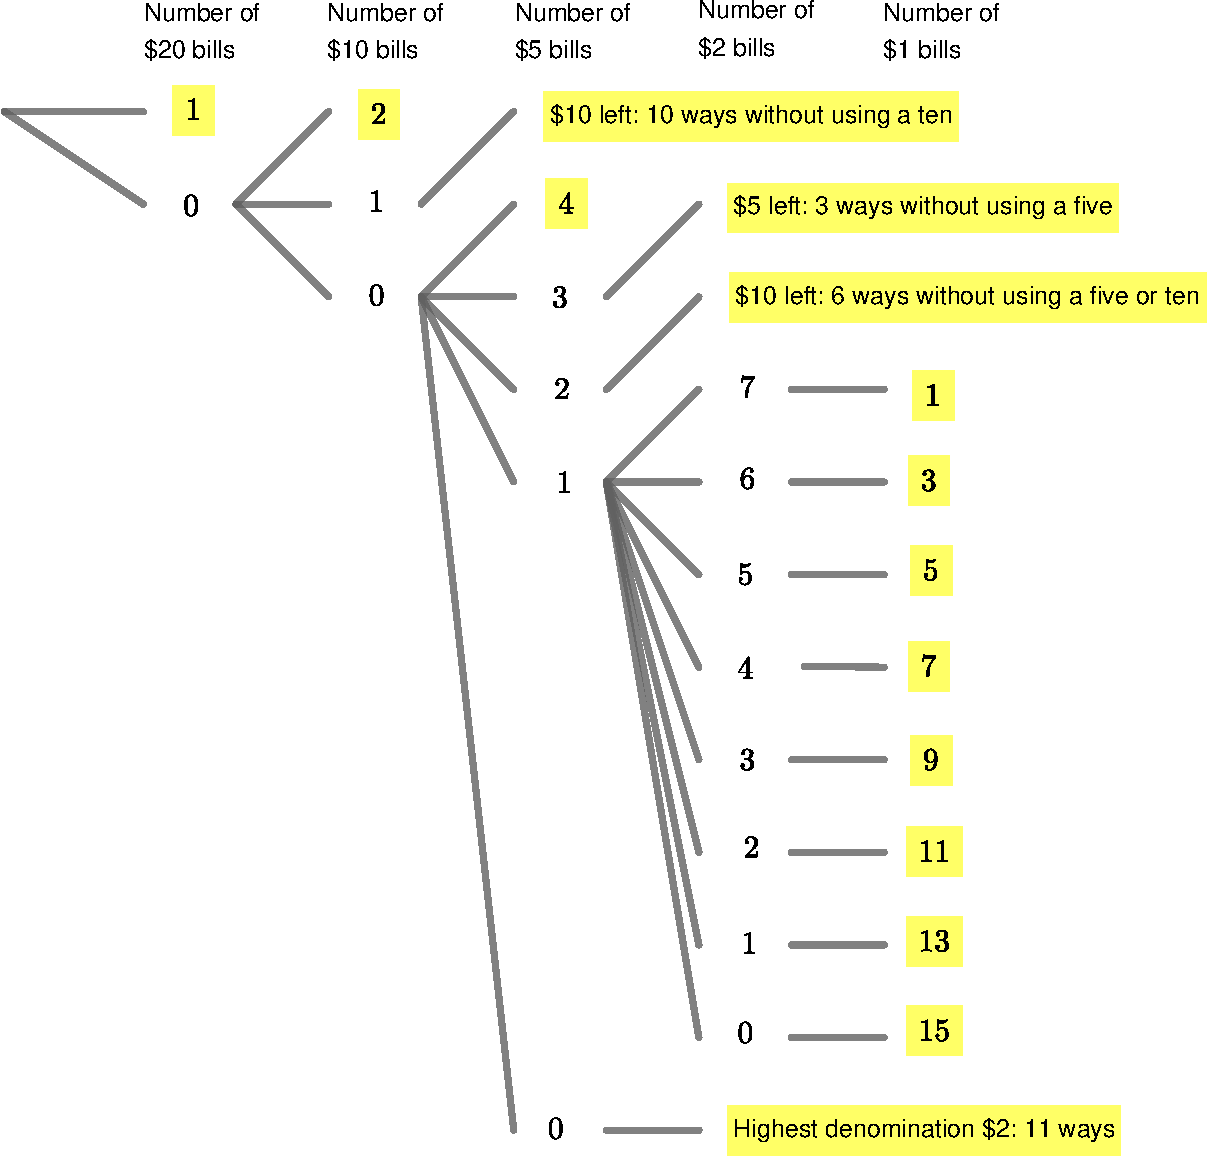
\includegraphics[width=5.5in]{images/Make20dollarsTree2.pdf}
    \end{center}
    }
    \par\Instr{ Another way to solve this problem is along the following lines.
    \begin{enumerate}
        \item \label{20withno10s} Determine the number of collections of bills that sum to \$20 and contain no \$20 bills or \$10 bills.
        \par
        This question is asking about the branches that do not begin with a \$10 or \$20 bill. So the first bill in each collection is below 10 and so the tree diagram will begin with three branches and proceed accordingly.
        \par The full tree diagram should look something like what is shown in Figure\ref{Making20Tree} producing $29$ total collections with no \$10 or \$20 bills. Notice there are key aspects of this tree that are worth exploring. Two key aspects mentioned above are:
        \begin{enumerate}
            \item Each branch has a bill denomination less than or equal to the branch it is stemming from.
            \item the branches that first use a \$5 bill must have a \$1 or another\$5 bill because of the necessity of an even number of odd denomination bills.
        \end{enumerate}
        \begin{figure}[htb]
            \begin{center}
                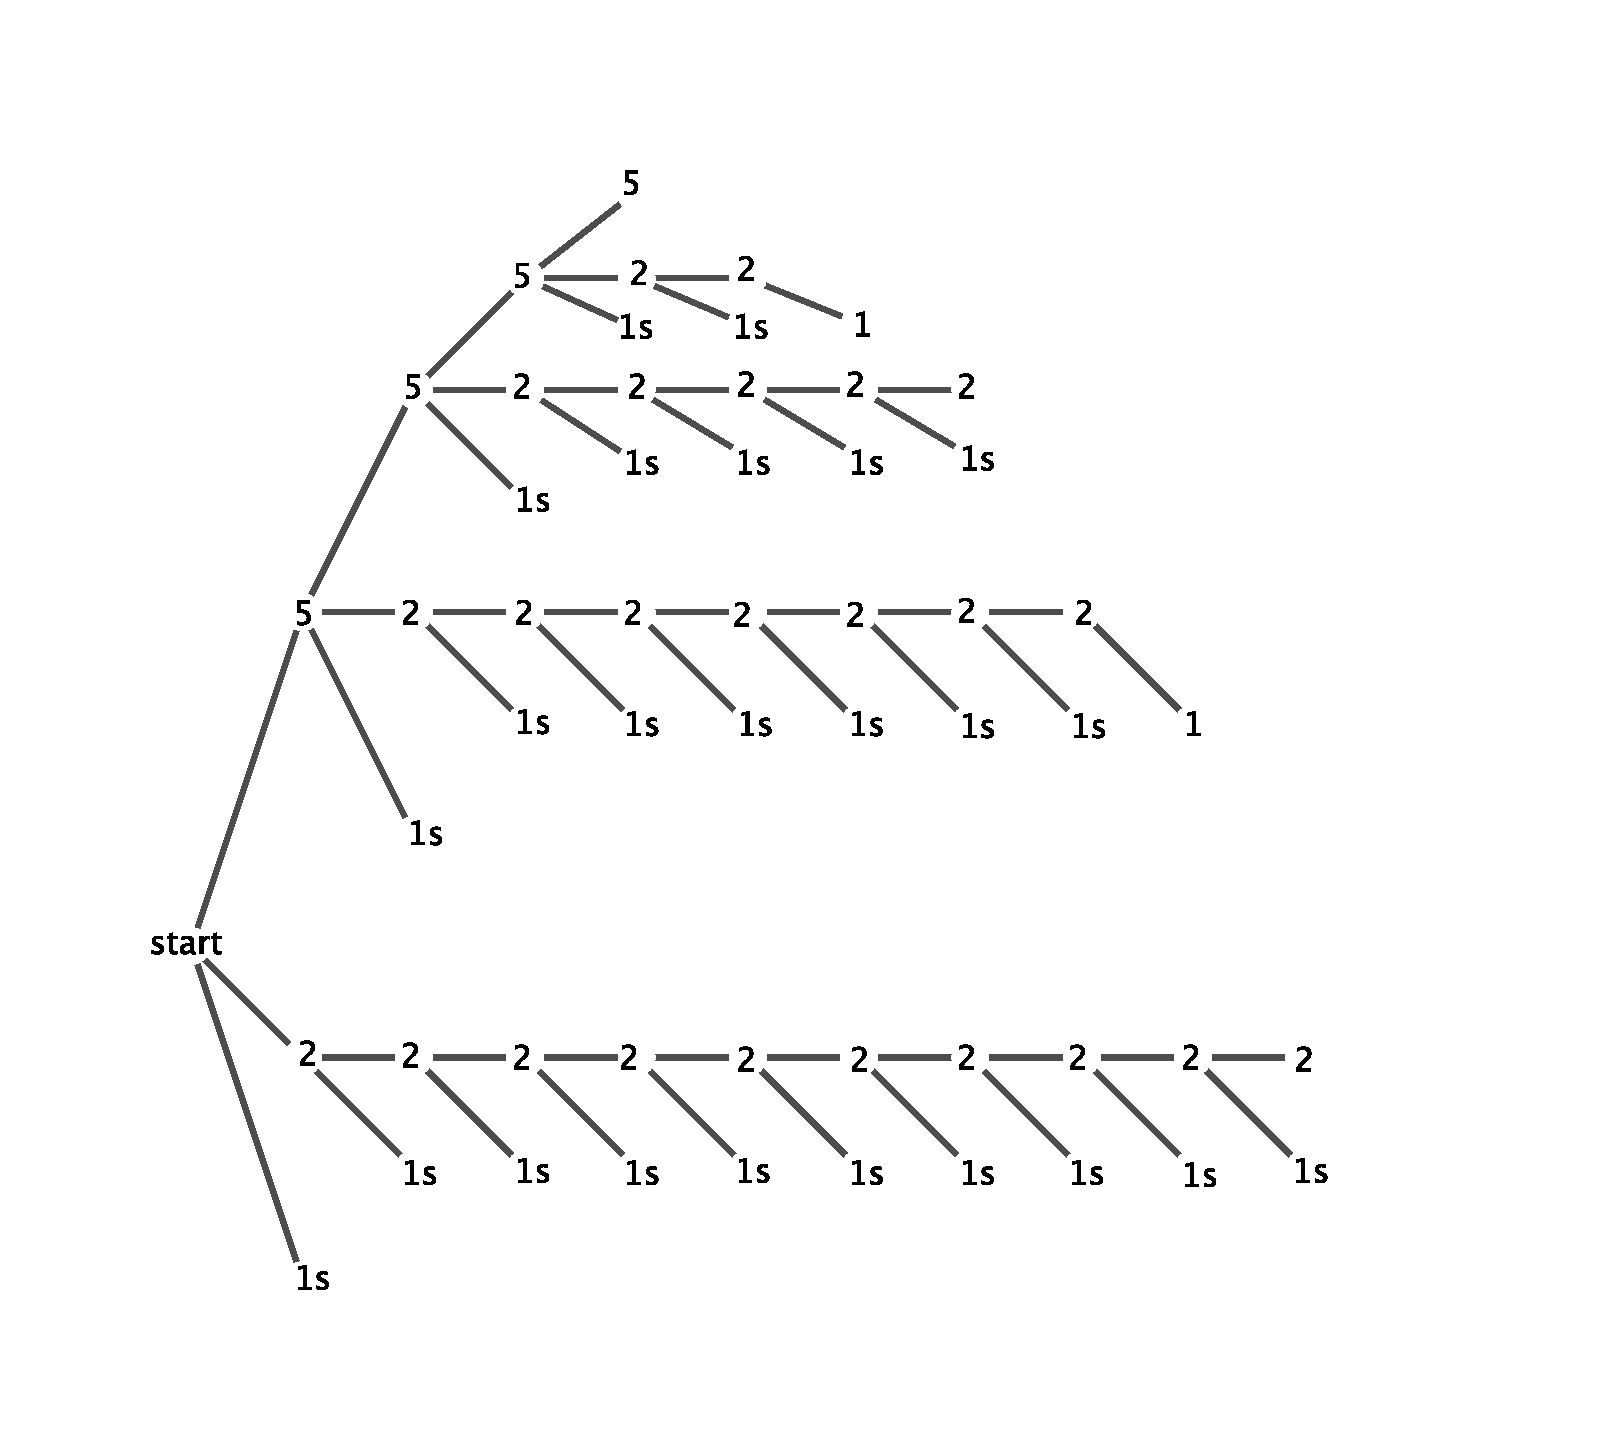
\includegraphics[width=5in]{images/Making20Tree.pdf}
            \end{center}
            \caption{ The entire solution tree for \$20 with no \$10 or \$20 bills}\label{Making20Tree}
        \end{figure}
        \item \label{20witha10} Determine the number of collections of bills that sum to \$20 and contain a \$10 bill.
        \par For the tree diagram organization method, this question is asking about the branch that begins with a \$10 bill. 
        \par We could create a tree diagram for this, but the existence of a \$10 bill leave us with needing a collection of ten more dollars. This was already solved in \ref{making10}. Therefore we know there are 11 collections of bills making up $20$ dollars that include a \$10 bill.
        \par Now the answers to the previous two questions can be added to the solution of using a single \$20 bill to solve the ultimate question. We get $1 + 29 + 11 = 41$ different ways to get a collection of bills that make \$20.
        \end{enumerate}
    }
    \wbvfill
    How many ways did you come up with?
    \par\Instr{ There are 41 ways. Counting the highlighted branches in the tree diagram above, there are 11 individual collections plus $10+3+6+11=30$ more for a total of 41.}
    \wbnewpage
    \item \textbf{Review the solution.}
    \begin{enumerate}
        \item How do you know you have not counted any collection more than once? In other words, how do you know each of your collections is different?
        \par\Instr{ As before, hopefully this will be more insightful that just saying "I checked my lists and didn't see any duplicates." It must rely on the fact that the smaller problems solved are disjoint.}
        \wbvfill
        \item How do you know you have all collections that make \$20? How do you know you have not missed any?
        \par\Instr{ This may be a tougher question to answer depending on the plan devised and carried out. But is students follow the suggestion in the exercises it may be something like "We listed all the ways to make \$20 where the highest denomination is \$1, where the highest denomination is \$2, and so on with highest \$5, \$10, and \$20. There are no other choices because using higher denominations than \$20 will give a total greater than \$20."}
        \wbvfill
    \end{enumerate}
    If you can't answer these questions or you have doubts that you have the correct answer you may need to revise your plan or how you carried it out.
\end{enumerate}

\newpage
\subsection{Exit Slip}
\begin{enumerate}
    \item How many different ways can you have \$15 in US bills? Provide a tree diagram, an organized list, or written justification for your answer.
    \par\Instr{ There are 22.
        \begin{center}
            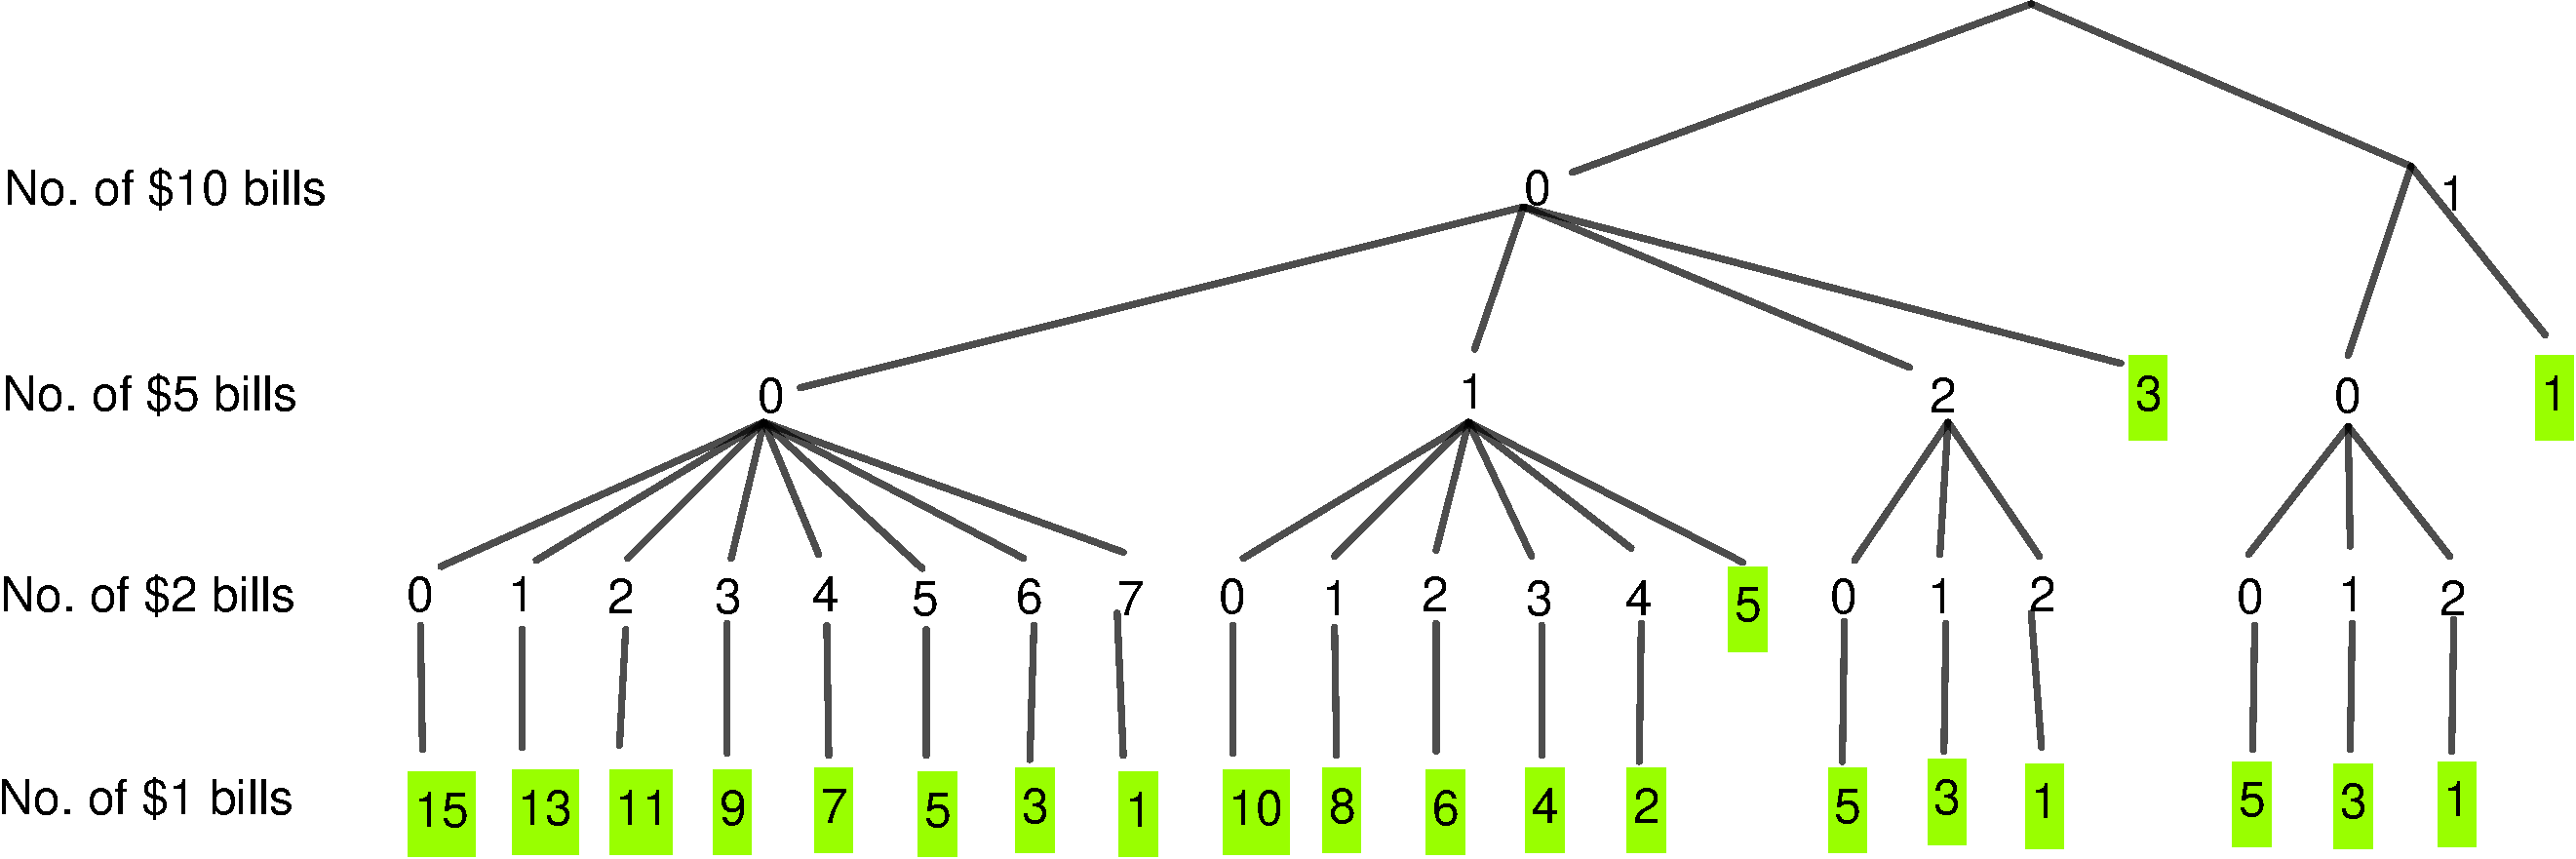
\includegraphics[scale=0.3]{images/Tree-FifteenDollars.pdf}
        \end{center}
    }
 \wbvfill
 
    \item At Panera Bread, you are presented with the following lunch choices: a starter of soup or salad; 3 different sandwiches; and a side of bread, chips, or an apple. How many different lunches consisting of one starter, one sandwich, and one side can be made?
        \par\Instr{ There are 18. This one can be calculated using the multiplication principle: $2\times 3\times 3=18$.
            \begin{center}
                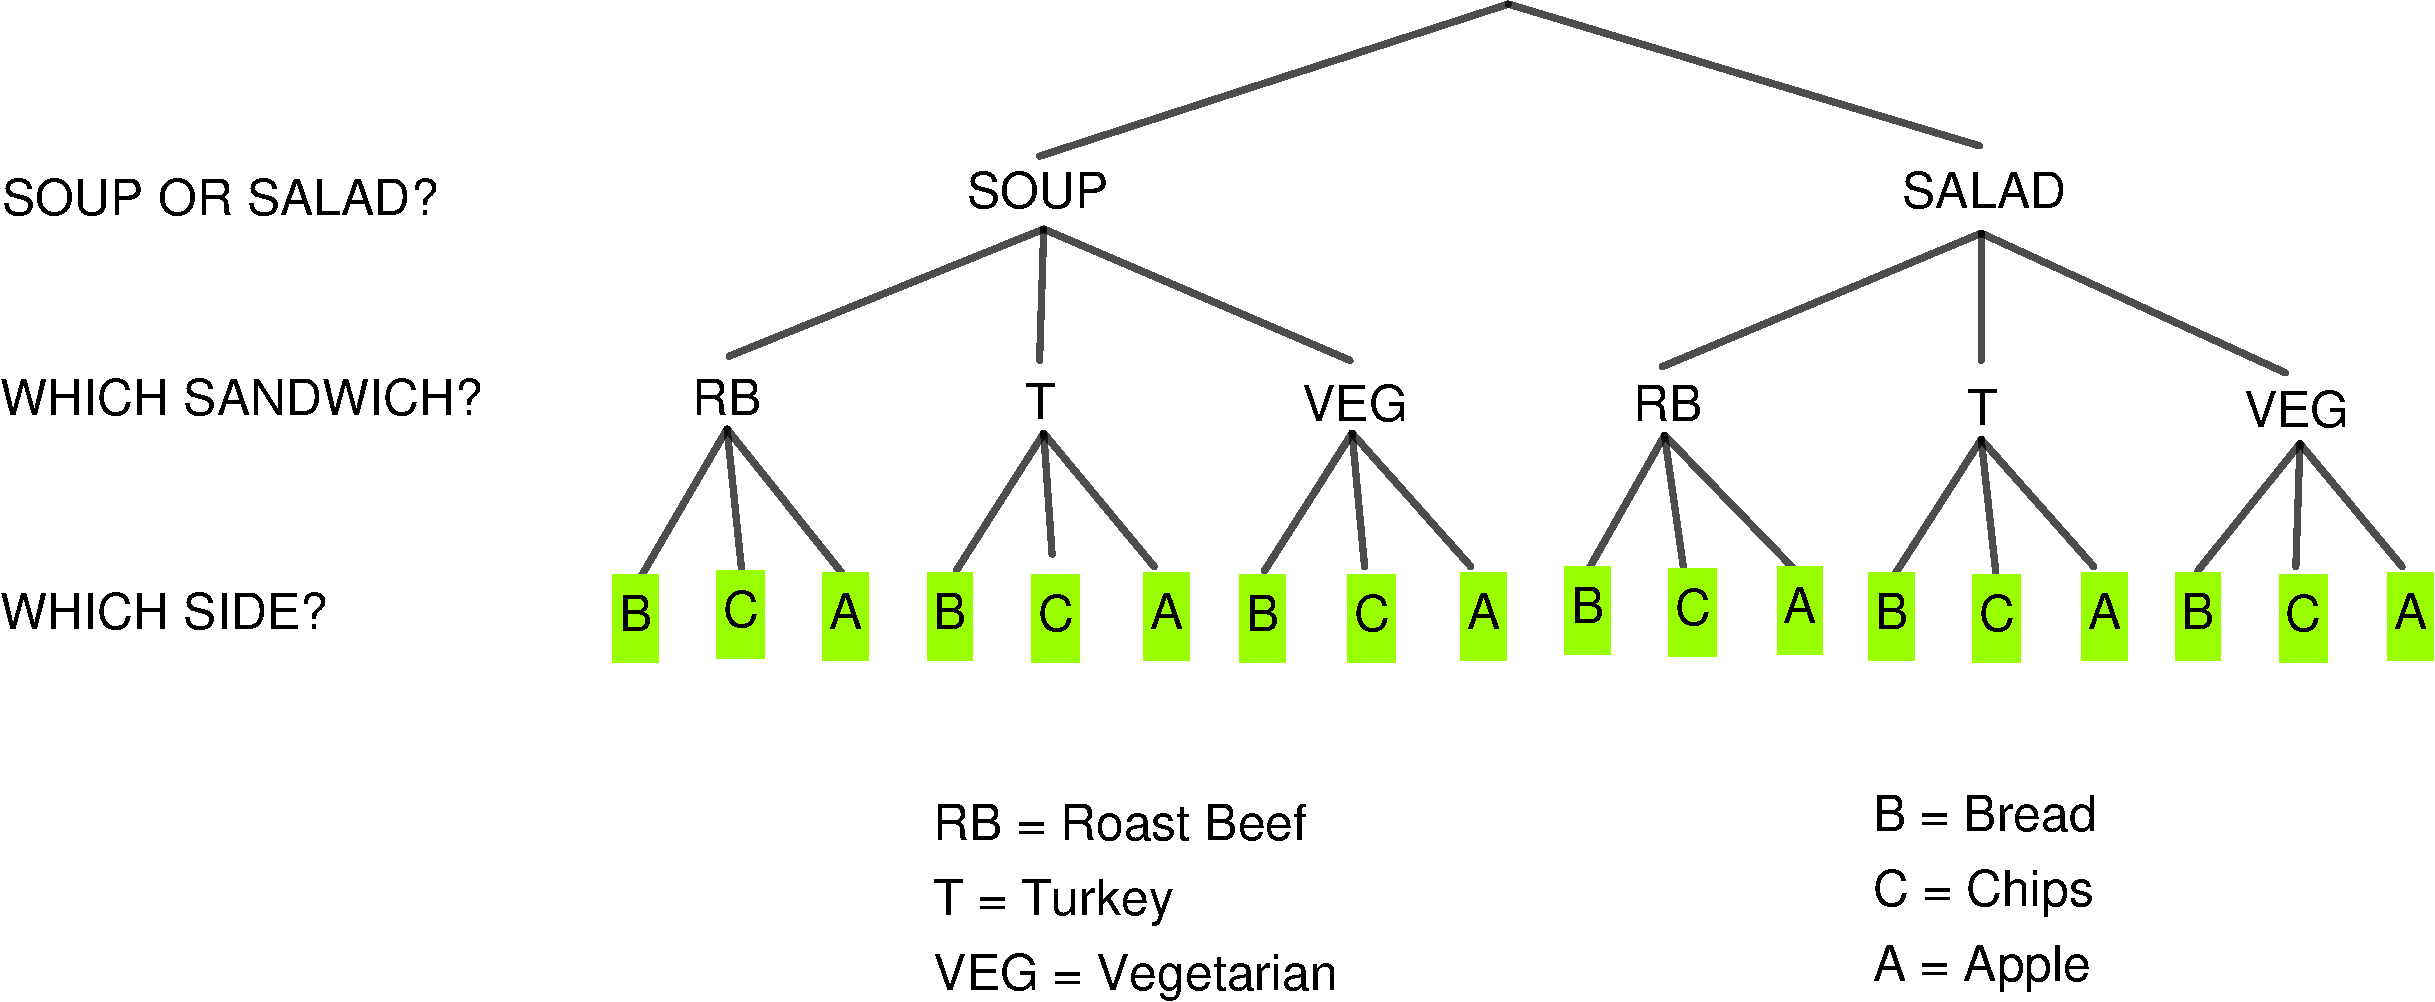
\includegraphics[scale=0.3]{images/Tree-Panera.pdf}
            \end{center}
        }
        
\wbvfill
\end{enumerate}


%%%%%%%%%%%%%%%
% Project %
%%%%%%%%%%%%%%%
\newpage
\section{Project Choices}

\begin{enumerate}
\item How many different ways can you make \$30 in US bills? Provide a tree diagram to support your claim and write a statement about how you used results from the \$20 class activity to find your answer.

\par\Instr{ One may initially think that you can multiply the number of ways to make \$10 by the number of ways to make \$20. However that drastically over counts the possibilities because the tree diagram resulting from this method would not produce unique branches.
    \par
    So without some advance counting techniques we will need to use an exhaustive counting method. However we will utilize some information we already have produced above.
    \par
    We will partition the solution set into those that have a \$20 bill and those that do not. For those that do have a \$20 bill, we know that we need ten more dollars and so the \$20 bill with all the solutions from question \ref{making10} will produce all 11 of the collections of bills containing a \$20 bill that add to \$30. 
    \par
    The harder part is to find the collection of bills that do not contain a \$20 bill. There are many ways to do this, but we would suggest partitioning this work into those that contain a \$10 bill and those that do not. For those that do, we know there is a \$10 bill so there are \$20 left to account for. Without using a \$20 bill there are 40 ways to make \$20, as we have seen. It is only left to find how many ways there are to make \$30 using only fives, twos, and ones. Making a tree diagram for these collections reveals 58 possibilities.
    \par
    Finally we would add all the possibilities from above to get $11+40+58 = 109$ total collections of U.S. bills that make \$30.}

\item At Domino's Pizza, the following unusual vegetable toppings are available: jalapeno peppers, roasted red peppers, spinach, and basil. How many different unusual veggie pizzas can you make using these toppings?
        \par\Instr{ There are 15. The N-N-N-N branch has none of the toppings so does not qualify as an unusual pizza. It is just plain cheese!
            \begin{center}
                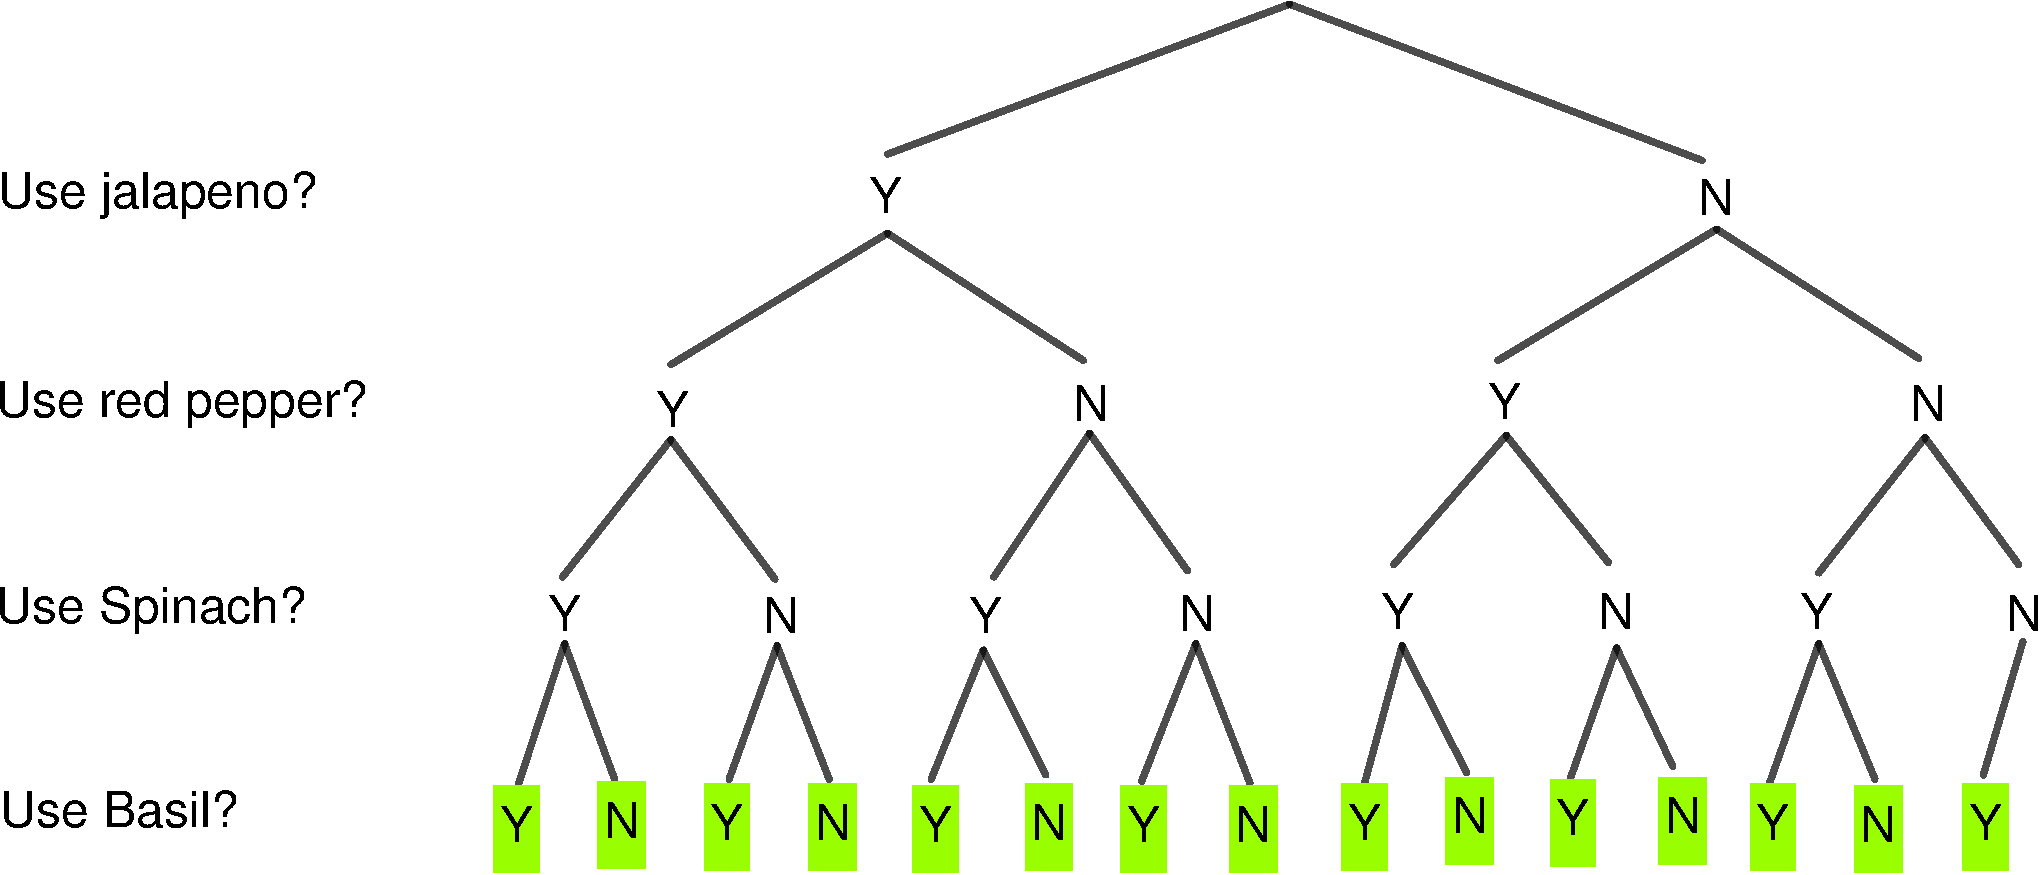
\includegraphics[scale=0.3]{images/Tree-Pizza.pdf}
            \end{center}
        }

 \item The division championship in major league baseball goes to the winner of a best-of-5 series. The first team to win 3 games wins the division, so the series will never go more than 5 games. For example, if the teams are Boston and Tampa Bay (as they were in the 2021 American League Division Series), one way it could have unfolded was B-T-B-T-T, meaning Boston won the first, Tampa Bay won second, Boston won the third, and then Tampa Bay won the fourth and fifth games. It also could have unfolded T-B-B-B (and this is what actually happened in 2021). How many different ways could the division series have unfolded (including the two already mentioned)?
        \par\Instr{ There are 20.
            \begin{center}
                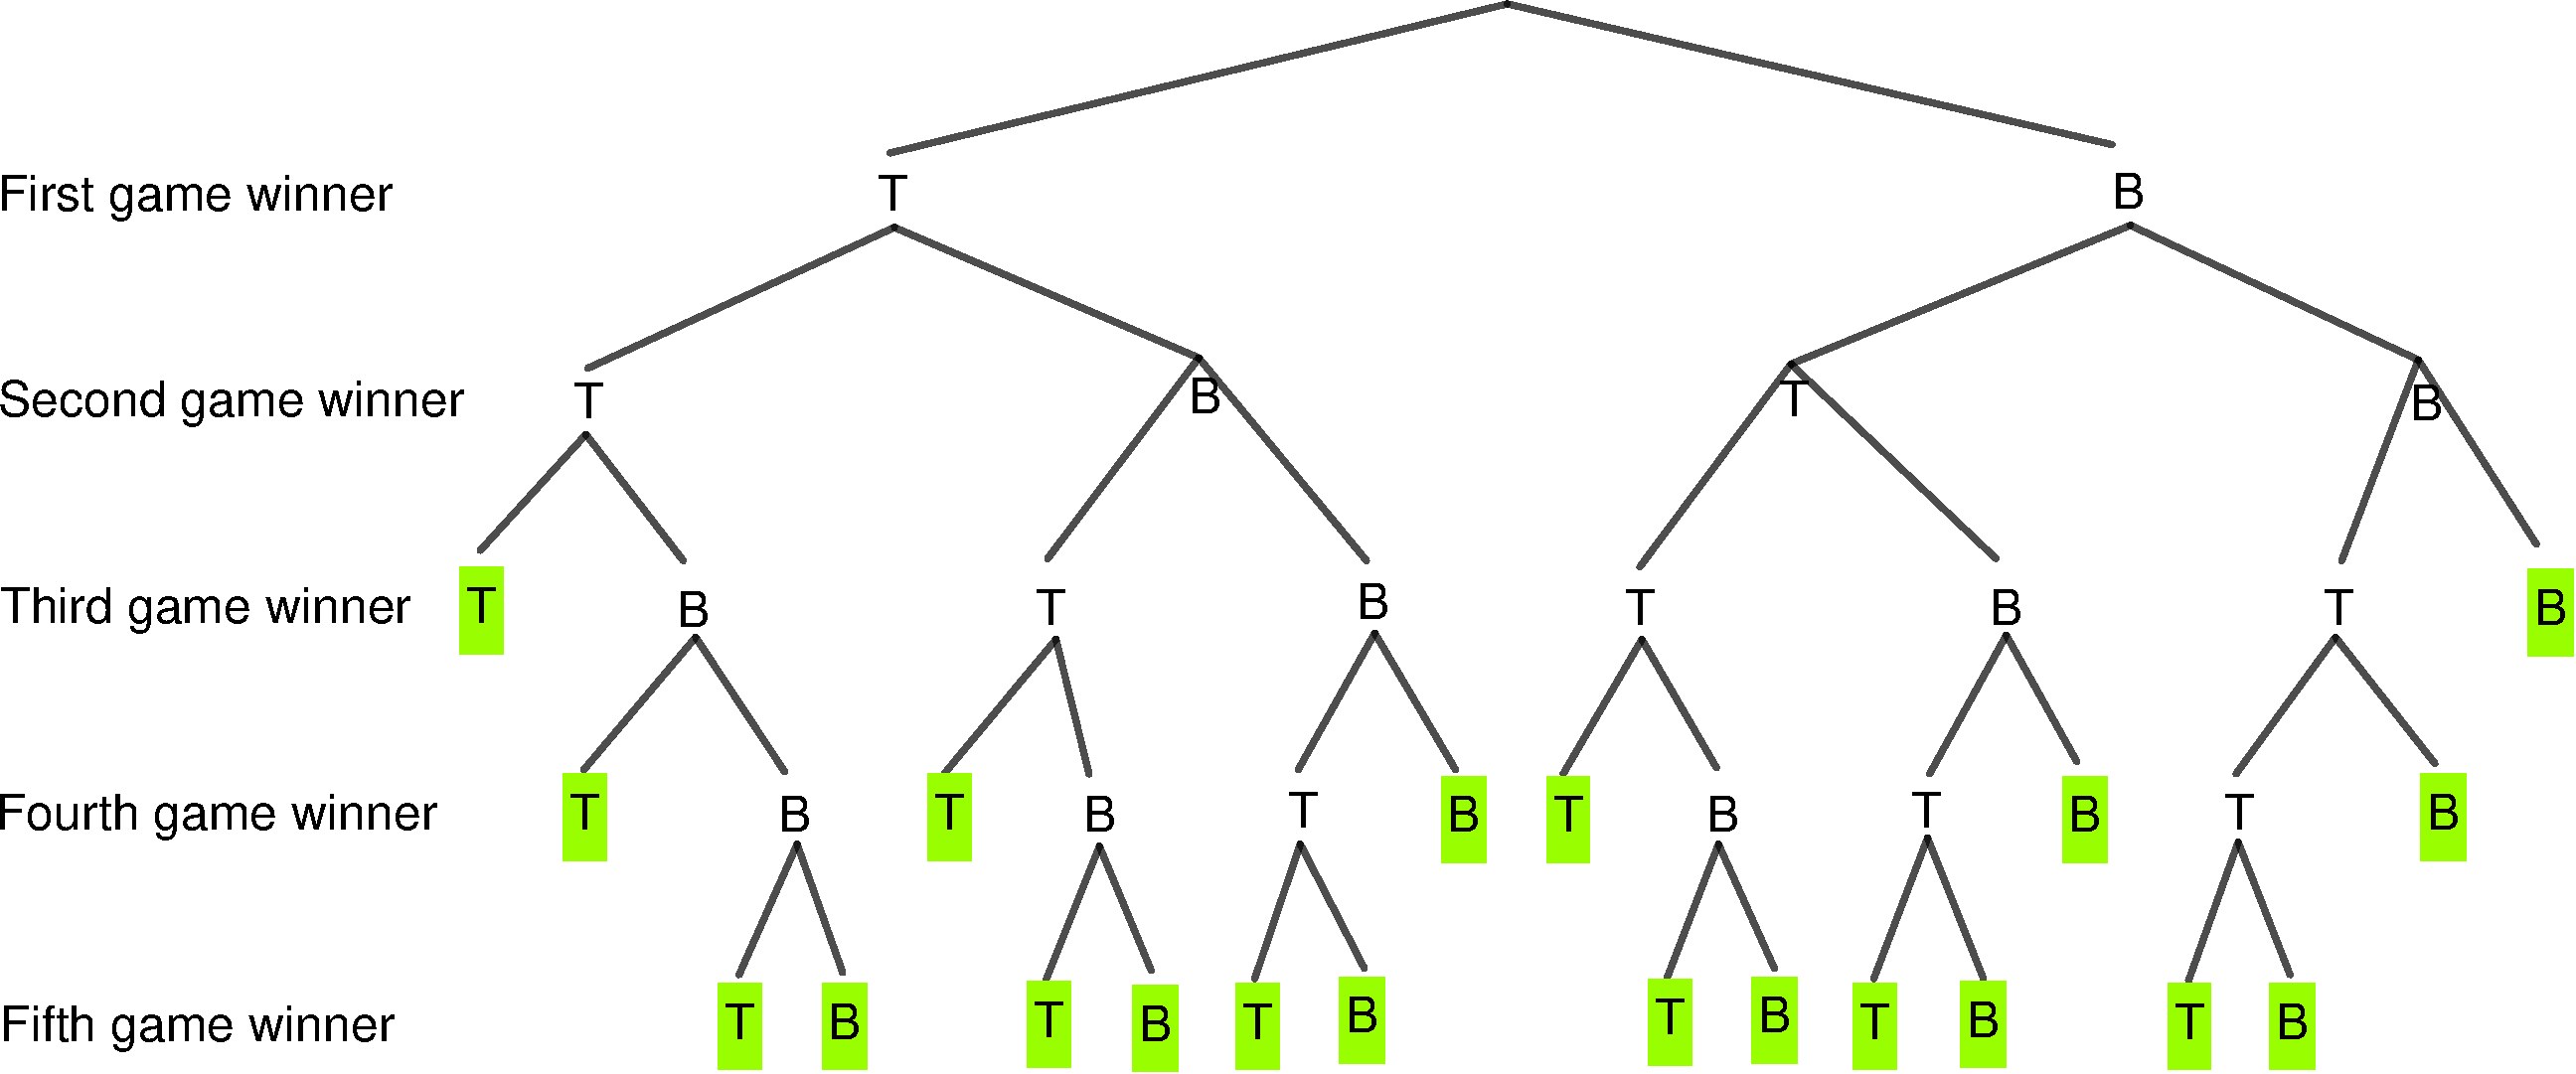
\includegraphics[scale=0.3]{images/Tree-DivisionSeries.pdf}
            \end{center}
        }

\item The curator at a natural history museum is designing a penguin display. He would like to put penguins of 4 different species in the display---Emperor, Northern Rockhopper, Macaroni, and African---arranged one next to the other in a row. However, he wants to be sure the Emperor Penguin is not next to the Macaroni Penguin. How many ways can he arrange the penguins in the display?
        \par\Instr{ There are 12.
            \begin{center}
                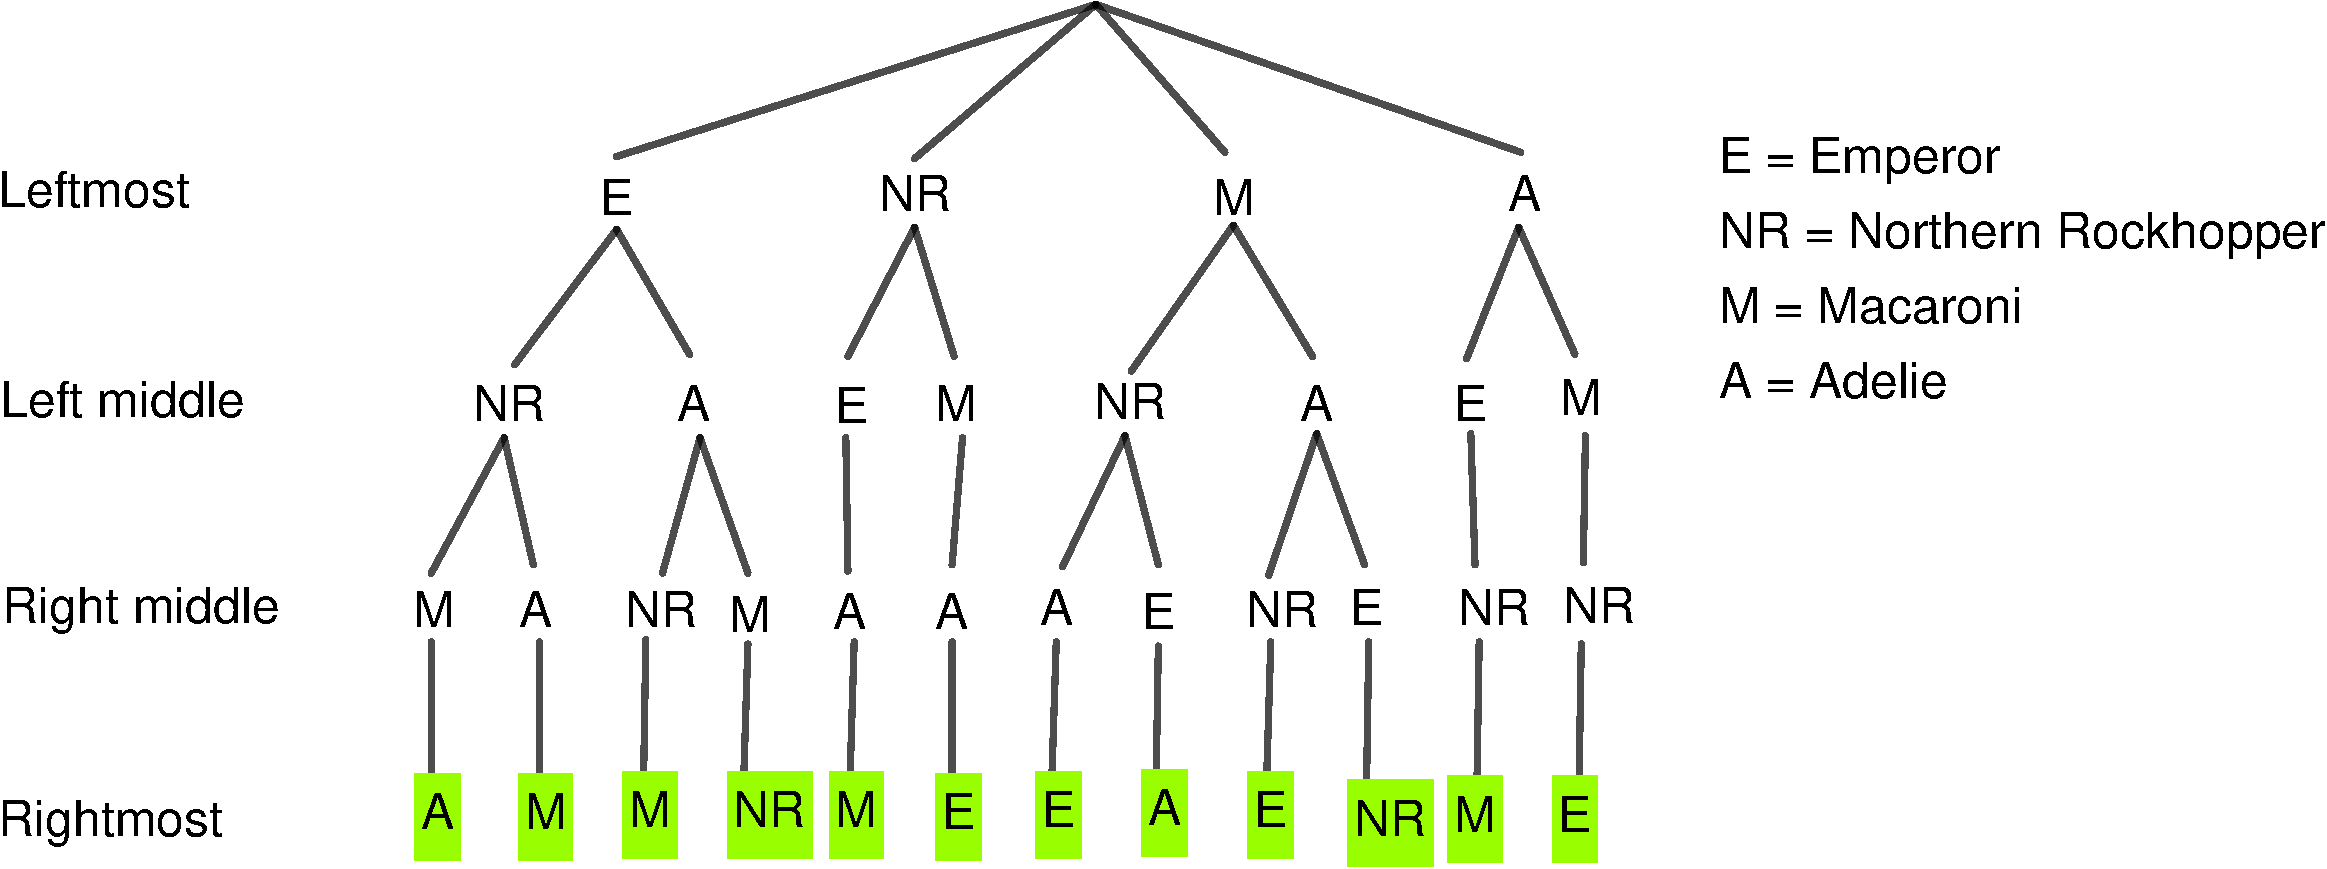
\includegraphics[scale=0.3]{images/Tree-Penguins.pdf}
            \end{center}
        }
    \end{enumerate}





\newpage
\section{Additional Exercises}
\begin{enumerate}
\item How many different ways can you make \$50 in US bills? Provide a tree diagram to support your claim and write a statement about how you used results from the \$20 class activity to find your answer.
\par\Instr{ The problem using coins to make a dollar is widely known, and I can find an answer for making \$50 with change but that number is extremely high because of the use of coins. We are asking for much less and the answer doesn't seem to be immediately available on the net.
\par
There are 451:
\begin{longtable}[c]{|c|c|c|c|c|c||c|c|c|c|c|c|}
\hline
50s & 20s & 10s & 5s & 2s & 1s & 50s & 20s & 10s & 5s & 2s & 1s \\ \hline\hline
0 & 0 & 0 & 0 & 0 & 50 &
0 & 0 & 0 & 0 & 1 & 48 \\ \hline
0 & 0 & 0 & 0 & 2 & 46 &
0 & 0 & 0 & 0 & 3 & 44 \\ \hline
0 & 0 & 0 & 0 & 4 & 42 &
0 & 0 & 0 & 0 & 5 & 40 \\ \hline
0 & 0 & 0 & 0 & 6 & 38 &
0 & 0 & 0 & 0 & 7 & 36 \\ \hline
0 & 0 & 0 & 0 & 8 & 34 &
0 & 0 & 0 & 0 & 9 & 32 \\ \hline
0 & 0 & 0 & 0 & 10 & 30 &
0 & 0 & 0 & 0 & 11 & 28 \\ \hline
0 & 0 & 0 & 0 & 12 & 26 &
0 & 0 & 0 & 0 & 13 & 24 \\ \hline
0 & 0 & 0 & 0 & 14 & 22 &
0 & 0 & 0 & 0 & 15 & 20 \\ \hline
0 & 0 & 0 & 0 & 16 & 18 &
0 & 0 & 0 & 0 & 17 & 16 \\ \hline
0 & 0 & 0 & 0 & 18 & 14 &
0 & 0 & 0 & 0 & 19 & 12 \\ \hline
0 & 0 & 0 & 0 & 20 & 10 &
0 & 0 & 0 & 0 & 21 & 8 \\ \hline
0 & 0 & 0 & 0 & 22 & 6 &
0 & 0 & 0 & 0 & 23 & 4 \\ \hline
0 & 0 & 0 & 0 & 24 & 2 &
0 & 0 & 0 & 0 & 25 & 0 \\ \hline
0 & 0 & 0 & 1 & 0 & 45 &
0 & 0 & 0 & 1 & 1 & 43 \\ \hline
0 & 0 & 0 & 1 & 2 & 41 &
0 & 0 & 0 & 1 & 3 & 39 \\ \hline
0 & 0 & 0 & 1 & 4 & 37 &
0 & 0 & 0 & 1 & 5 & 35 \\ \hline
0 & 0 & 0 & 1 & 6 & 33 &
0 & 0 & 0 & 1 & 7 & 31 \\ \hline
0 & 0 & 0 & 1 & 8 & 29 &
0 & 0 & 0 & 1 & 9 & 27 \\ \hline
0 & 0 & 0 & 1 & 10 & 25 &
0 & 0 & 0 & 1 & 11 & 23 \\ \hline
0 & 0 & 0 & 1 & 12 & 21 &
0 & 0 & 0 & 1 & 13 & 19 \\ \hline
0 & 0 & 0 & 1 & 14 & 17 &
0 & 0 & 0 & 1 & 15 & 15 \\ \hline
0 & 0 & 0 & 1 & 16 & 13 &
0 & 0 & 0 & 1 & 17 & 11 \\ \hline
0 & 0 & 0 & 1 & 18 & 9 &
0 & 0 & 0 & 1 & 19 & 7 \\ \hline
0 & 0 & 0 & 1 & 20 & 5 &
0 & 0 & 0 & 1 & 21 & 3 \\ \hline
0 & 0 & 0 & 1 & 22 & 1 &
0 & 0 & 0 & 2 & 0 & 40 \\ \hline
0 & 0 & 0 & 2 & 1 & 38 &
0 & 0 & 0 & 2 & 2 & 36 \\ \hline
0 & 0 & 0 & 2 & 3 & 34 &
0 & 0 & 0 & 2 & 4 & 32 \\ \hline
0 & 0 & 0 & 2 & 5 & 30 &
0 & 0 & 0 & 2 & 6 & 28 \\ \hline
0 & 0 & 0 & 2 & 7 & 26 &
0 & 0 & 0 & 2 & 8 & 24 \\ \hline
0 & 0 & 0 & 2 & 9 & 22 &
0 & 0 & 0 & 2 & 10 & 20 \\ \hline
0 & 0 & 0 & 2 & 11 & 18 &
0 & 0 & 0 & 2 & 12 & 16 \\ \hline
0 & 0 & 0 & 2 & 13 & 14 &
0 & 0 & 0 & 2 & 14 & 12 \\ \hline
0 & 0 & 0 & 2 & 15 & 10 &
0 & 0 & 0 & 2 & 16 & 8 \\ \hline
0 & 0 & 0 & 2 & 17 & 6 &
0 & 0 & 0 & 2 & 18 & 4 \\ \hline
0 & 0 & 0 & 2 & 19 & 2 &
0 & 0 & 0 & 2 & 20 & 0 \\ \hline
0 & 0 & 0 & 3 & 0 & 35 &
0 & 0 & 0 & 3 & 1 & 33 \\ \hline
0 & 0 & 0 & 3 & 2 & 31 &
0 & 0 & 0 & 3 & 3 & 29 \\ \hline
0 & 0 & 0 & 3 & 4 & 27 &
0 & 0 & 0 & 3 & 5 & 25 \\ \hline
0 & 0 & 0 & 3 & 6 & 23 &
0 & 0 & 0 & 3 & 7 & 21 \\ \hline
0 & 0 & 0 & 3 & 8 & 19 &
0 & 0 & 0 & 3 & 9 & 17 \\ \hline
0 & 0 & 0 & 3 & 10 & 15 &
0 & 0 & 0 & 3 & 11 & 13 \\ \hline
0 & 0 & 0 & 3 & 12 & 11 &
0 & 0 & 0 & 3 & 13 & 9 \\ \hline
0 & 0 & 0 & 3 & 14 & 7 &
0 & 0 & 0 & 3 & 15 & 5 \\ \hline
0 & 0 & 0 & 3 & 16 & 3 &
0 & 0 & 0 & 3 & 17 & 1 \\ \hline
0 & 0 & 0 & 4 & 0 & 30 &
0 & 0 & 0 & 4 & 1 & 28 \\ \hline
0 & 0 & 0 & 4 & 2 & 26 &
0 & 0 & 0 & 4 & 3 & 24 \\ \hline
0 & 0 & 0 & 4 & 4 & 22 &
0 & 0 & 0 & 4 & 5 & 20 \\ \hline
0 & 0 & 0 & 4 & 6 & 18 &
0 & 0 & 0 & 4 & 7 & 16 \\ \hline
0 & 0 & 0 & 4 & 8 & 14 &
0 & 0 & 0 & 4 & 9 & 12 \\ \hline
0 & 0 & 0 & 4 & 10 & 10 &
0 & 0 & 0 & 4 & 11 & 8 \\ \hline
0 & 0 & 0 & 4 & 12 & 6 &
0 & 0 & 0 & 4 & 13 & 4 \\ \hline
0 & 0 & 0 & 4 & 14 & 2 &
0 & 0 & 0 & 4 & 15 & 0 \\ \hline
0 & 0 & 0 & 5 & 0 & 25 &
0 & 0 & 0 & 5 & 1 & 23 \\ \hline
0 & 0 & 0 & 5 & 2 & 21 &
0 & 0 & 0 & 5 & 3 & 19 \\ \hline
0 & 0 & 0 & 5 & 4 & 17 &
0 & 0 & 0 & 5 & 5 & 15 \\ \hline
0 & 0 & 0 & 5 & 6 & 13 &
0 & 0 & 0 & 5 & 7 & 11 \\ \hline
0 & 0 & 0 & 5 & 8 & 9 &
0 & 0 & 0 & 5 & 9 & 7 \\ \hline
0 & 0 & 0 & 5 & 10 & 5 &
0 & 0 & 0 & 5 & 11 & 3 \\ \hline
0 & 0 & 0 & 5 & 12 & 1 &
0 & 0 & 0 & 6 & 0 & 20 \\ \hline
0 & 0 & 0 & 6 & 1 & 18 &
0 & 0 & 0 & 6 & 2 & 16 \\ \hline
0 & 0 & 0 & 6 & 3 & 14 &
0 & 0 & 0 & 6 & 4 & 12 \\ \hline
0 & 0 & 0 & 6 & 5 & 10 &
0 & 0 & 0 & 6 & 6 & 8 \\ \hline
0 & 0 & 0 & 6 & 7 & 6 &
0 & 0 & 0 & 6 & 8 & 4 \\ \hline
0 & 0 & 0 & 6 & 9 & 2 &
0 & 0 & 0 & 6 & 10 & 0 \\ \hline
0 & 0 & 0 & 7 & 0 & 15 &
0 & 0 & 0 & 7 & 1 & 13 \\ \hline
0 & 0 & 0 & 7 & 2 & 11 &
0 & 0 & 0 & 7 & 3 & 9 \\ \hline
0 & 0 & 0 & 7 & 4 & 7 &
0 & 0 & 0 & 7 & 5 & 5 \\ \hline
0 & 0 & 0 & 7 & 6 & 3 &
0 & 0 & 0 & 7 & 7 & 1 \\ \hline
0 & 0 & 0 & 8 & 0 & 10 &
0 & 0 & 0 & 8 & 1 & 8 \\ \hline
0 & 0 & 0 & 8 & 2 & 6 &
0 & 0 & 0 & 8 & 3 & 4 \\ \hline
0 & 0 & 0 & 8 & 4 & 2 &
0 & 0 & 0 & 8 & 5 & 0 \\ \hline
0 & 0 & 0 & 9 & 0 & 5 &
0 & 0 & 0 & 9 & 1 & 3 \\ \hline
0 & 0 & 0 & 9 & 2 & 1 &
0 & 0 & 0 & 10 & 0 & 0 \\ \hline
0 & 0 & 1 & 0 & 0 & 40 &
0 & 0 & 1 & 0 & 1 & 38 \\ \hline
0 & 0 & 1 & 0 & 2 & 36 &
0 & 0 & 1 & 0 & 3 & 34 \\ \hline
0 & 0 & 1 & 0 & 4 & 32 &
0 & 0 & 1 & 0 & 5 & 30 \\ \hline
0 & 0 & 1 & 0 & 6 & 28 &
0 & 0 & 1 & 0 & 7 & 26 \\ \hline
0 & 0 & 1 & 0 & 8 & 24 &
0 & 0 & 1 & 0 & 9 & 22 \\ \hline
0 & 0 & 1 & 0 & 10 & 20 &
0 & 0 & 1 & 0 & 11 & 18 \\ \hline
0 & 0 & 1 & 0 & 12 & 16 &
0 & 0 & 1 & 0 & 13 & 14 \\ \hline
0 & 0 & 1 & 0 & 14 & 12 &
0 & 0 & 1 & 0 & 15 & 10 \\ \hline
0 & 0 & 1 & 0 & 16 & 8 &
0 & 0 & 1 & 0 & 17 & 6 \\ \hline
0 & 0 & 1 & 0 & 18 & 4 &
0 & 0 & 1 & 0 & 19 & 2 \\ \hline
0 & 0 & 1 & 0 & 20 & 0 &
0 & 0 & 1 & 1 & 0 & 35 \\ \hline
0 & 0 & 1 & 1 & 1 & 33 &
0 & 0 & 1 & 1 & 2 & 31 \\ \hline
0 & 0 & 1 & 1 & 3 & 29 &
0 & 0 & 1 & 1 & 4 & 27 \\ \hline
0 & 0 & 1 & 1 & 5 & 25 &
0 & 0 & 1 & 1 & 6 & 23 \\ \hline
0 & 0 & 1 & 1 & 7 & 21 &
0 & 0 & 1 & 1 & 8 & 19 \\ \hline
0 & 0 & 1 & 1 & 9 & 17 &
0 & 0 & 1 & 1 & 10 & 15 \\ \hline
0 & 0 & 1 & 1 & 11 & 13 &
0 & 0 & 1 & 1 & 12 & 11 \\ \hline
0 & 0 & 1 & 1 & 13 & 9 &
0 & 0 & 1 & 1 & 14 & 7 \\ \hline
0 & 0 & 1 & 1 & 15 & 5 &
0 & 0 & 1 & 1 & 16 & 3 \\ \hline
0 & 0 & 1 & 1 & 17 & 1 &
0 & 0 & 1 & 2 & 0 & 30 \\ \hline
0 & 0 & 1 & 2 & 1 & 28 &
0 & 0 & 1 & 2 & 2 & 26 \\ \hline
0 & 0 & 1 & 2 & 3 & 24 &
0 & 0 & 1 & 2 & 4 & 22 \\ \hline
0 & 0 & 1 & 2 & 5 & 20 &
0 & 0 & 1 & 2 & 6 & 18 \\ \hline
0 & 0 & 1 & 2 & 7 & 16 &
0 & 0 & 1 & 2 & 8 & 14 \\ \hline
0 & 0 & 1 & 2 & 9 & 12 &
0 & 0 & 1 & 2 & 10 & 10 \\ \hline
0 & 0 & 1 & 2 & 11 & 8 &
0 & 0 & 1 & 2 & 12 & 6 \\ \hline
0 & 0 & 1 & 2 & 13 & 4 &
0 & 0 & 1 & 2 & 14 & 2 \\ \hline
0 & 0 & 1 & 2 & 15 & 0 &
0 & 0 & 1 & 3 & 0 & 25 \\ \hline
0 & 0 & 1 & 3 & 1 & 23 &
0 & 0 & 1 & 3 & 2 & 21 \\ \hline
0 & 0 & 1 & 3 & 3 & 19 &
0 & 0 & 1 & 3 & 4 & 17 \\ \hline
0 & 0 & 1 & 3 & 5 & 15 &
0 & 0 & 1 & 3 & 6 & 13 \\ \hline
0 & 0 & 1 & 3 & 7 & 11 &
0 & 0 & 1 & 3 & 8 & 9 \\ \hline
0 & 0 & 1 & 3 & 9 & 7 &
0 & 0 & 1 & 3 & 10 & 5 \\ \hline
0 & 0 & 1 & 3 & 11 & 3 &
0 & 0 & 1 & 3 & 12 & 1 \\ \hline
0 & 0 & 1 & 4 & 0 & 20 &
0 & 0 & 1 & 4 & 1 & 18 \\ \hline
0 & 0 & 1 & 4 & 2 & 16 &
0 & 0 & 1 & 4 & 3 & 14 \\ \hline
0 & 0 & 1 & 4 & 4 & 12 &
0 & 0 & 1 & 4 & 5 & 10 \\ \hline
0 & 0 & 1 & 4 & 6 & 8 &
0 & 0 & 1 & 4 & 7 & 6 \\ \hline
0 & 0 & 1 & 4 & 8 & 4 &
0 & 0 & 1 & 4 & 9 & 2 \\ \hline
0 & 0 & 1 & 4 & 10 & 0 &
0 & 0 & 1 & 5 & 0 & 15 \\ \hline
0 & 0 & 1 & 5 & 1 & 13 &
0 & 0 & 1 & 5 & 2 & 11 \\ \hline
0 & 0 & 1 & 5 & 3 & 9 &
0 & 0 & 1 & 5 & 4 & 7 \\ \hline
0 & 0 & 1 & 5 & 5 & 5 &
0 & 0 & 1 & 5 & 6 & 3 \\ \hline
0 & 0 & 1 & 5 & 7 & 1 &
0 & 0 & 1 & 6 & 0 & 10 \\ \hline
0 & 0 & 1 & 6 & 1 & 8 &
0 & 0 & 1 & 6 & 2 & 6 \\ \hline
0 & 0 & 1 & 6 & 3 & 4 &
0 & 0 & 1 & 6 & 4 & 2 \\ \hline
0 & 0 & 1 & 6 & 5 & 0 &
0 & 0 & 1 & 7 & 0 & 5 \\ \hline
0 & 0 & 1 & 7 & 1 & 3 &
0 & 0 & 1 & 7 & 2 & 1 \\ \hline
0 & 0 & 1 & 8 & 0 & 0 &
0 & 0 & 2 & 0 & 0 & 30 \\ \hline
0 & 0 & 2 & 0 & 1 & 28 &
0 & 0 & 2 & 0 & 2 & 26 \\ \hline
0 & 0 & 2 & 0 & 3 & 24 &
0 & 0 & 2 & 0 & 4 & 22 \\ \hline
0 & 0 & 2 & 0 & 5 & 20 &
0 & 0 & 2 & 0 & 6 & 18 \\ \hline
0 & 0 & 2 & 0 & 7 & 16 &
0 & 0 & 2 & 0 & 8 & 14 \\ \hline
0 & 0 & 2 & 0 & 9 & 12 &
0 & 0 & 2 & 0 & 10 & 10 \\ \hline
0 & 0 & 2 & 0 & 11 & 8 &
0 & 0 & 2 & 0 & 12 & 6 \\ \hline
0 & 0 & 2 & 0 & 13 & 4 &
0 & 0 & 2 & 0 & 14 & 2 \\ \hline
0 & 0 & 2 & 0 & 15 & 0 &
0 & 0 & 2 & 1 & 0 & 25 \\ \hline
0 & 0 & 2 & 1 & 1 & 23 &
0 & 0 & 2 & 1 & 2 & 21 \\ \hline
0 & 0 & 2 & 1 & 3 & 19 &
0 & 0 & 2 & 1 & 4 & 17 \\ \hline
0 & 0 & 2 & 1 & 5 & 15 &
0 & 0 & 2 & 1 & 6 & 13 \\ \hline
0 & 0 & 2 & 1 & 7 & 11 &
0 & 0 & 2 & 1 & 8 & 9 \\ \hline
0 & 0 & 2 & 1 & 9 & 7 &
0 & 0 & 2 & 1 & 10 & 5 \\ \hline
0 & 0 & 2 & 1 & 11 & 3 &
0 & 0 & 2 & 1 & 12 & 1 \\ \hline
0 & 0 & 2 & 2 & 0 & 20 &
0 & 0 & 2 & 2 & 1 & 18 \\ \hline
0 & 0 & 2 & 2 & 2 & 16 &
0 & 0 & 2 & 2 & 3 & 14 \\ \hline
0 & 0 & 2 & 2 & 4 & 12 &
0 & 0 & 2 & 2 & 5 & 10 \\ \hline
0 & 0 & 2 & 2 & 6 & 8 &
0 & 0 & 2 & 2 & 7 & 6 \\ \hline
0 & 0 & 2 & 2 & 8 & 4 &
0 & 0 & 2 & 2 & 9 & 2 \\ \hline
0 & 0 & 2 & 2 & 10 & 0 &
0 & 0 & 2 & 3 & 0 & 15 \\ \hline
0 & 0 & 2 & 3 & 1 & 13 &
0 & 0 & 2 & 3 & 2 & 11 \\ \hline
0 & 0 & 2 & 3 & 3 & 9 &
0 & 0 & 2 & 3 & 4 & 7 \\ \hline
0 & 0 & 2 & 3 & 5 & 5 &
0 & 0 & 2 & 3 & 6 & 3 \\ \hline
0 & 0 & 2 & 3 & 7 & 1 &
0 & 0 & 2 & 4 & 0 & 10 \\ \hline
0 & 0 & 2 & 4 & 1 & 8 &
0 & 0 & 2 & 4 & 2 & 6 \\ \hline
0 & 0 & 2 & 4 & 3 & 4 &
0 & 0 & 2 & 4 & 4 & 2 \\ \hline
0 & 0 & 2 & 4 & 5 & 0 &
0 & 0 & 2 & 5 & 0 & 5 \\ \hline
0 & 0 & 2 & 5 & 1 & 3 &
0 & 0 & 2 & 5 & 2 & 1 \\ \hline
0 & 0 & 2 & 6 & 0 & 0 &
0 & 0 & 3 & 0 & 0 & 20 \\ \hline
0 & 0 & 3 & 0 & 1 & 18 &
0 & 0 & 3 & 0 & 2 & 16 \\ \hline
0 & 0 & 3 & 0 & 3 & 14 &
0 & 0 & 3 & 0 & 4 & 12 \\ \hline
0 & 0 & 3 & 0 & 5 & 10 &
0 & 0 & 3 & 0 & 6 & 8 \\ \hline
0 & 0 & 3 & 0 & 7 & 6 &
0 & 0 & 3 & 0 & 8 & 4 \\ \hline
0 & 0 & 3 & 0 & 9 & 2 &
0 & 0 & 3 & 0 & 10 & 0 \\ \hline
0 & 0 & 3 & 1 & 0 & 15 &
0 & 0 & 3 & 1 & 1 & 13 \\ \hline
0 & 0 & 3 & 1 & 2 & 11 &
0 & 0 & 3 & 1 & 3 & 9 \\ \hline
0 & 0 & 3 & 1 & 4 & 7 &
0 & 0 & 3 & 1 & 5 & 5 \\ \hline
0 & 0 & 3 & 1 & 6 & 3 &
0 & 0 & 3 & 1 & 7 & 1 \\ \hline
0 & 0 & 3 & 2 & 0 & 10 &
0 & 0 & 3 & 2 & 1 & 8 \\ \hline
0 & 0 & 3 & 2 & 2 & 6 &
0 & 0 & 3 & 2 & 3 & 4 \\ \hline
0 & 0 & 3 & 2 & 4 & 2 &
0 & 0 & 3 & 2 & 5 & 0 \\ \hline
0 & 0 & 3 & 3 & 0 & 5 &
0 & 0 & 3 & 3 & 1 & 3 \\ \hline
0 & 0 & 3 & 3 & 2 & 1 &
0 & 0 & 3 & 4 & 0 & 0 \\ \hline
0 & 0 & 4 & 0 & 0 & 10 &
0 & 0 & 4 & 0 & 1 & 8 \\ \hline
0 & 0 & 4 & 0 & 2 & 6 &
0 & 0 & 4 & 0 & 3 & 4 \\ \hline
0 & 0 & 4 & 0 & 4 & 2 &
0 & 0 & 4 & 0 & 5 & 0 \\ \hline
0 & 0 & 4 & 1 & 0 & 5 &
0 & 0 & 4 & 1 & 1 & 3 \\ \hline
0 & 0 & 4 & 1 & 2 & 1 &
0 & 0 & 4 & 2 & 0 & 0 \\ \hline
0 & 0 & 5 & 0 & 0 & 0 &
0 & 1 & 0 & 0 & 0 & 30 \\ \hline
0 & 1 & 0 & 0 & 1 & 28 &
0 & 1 & 0 & 0 & 2 & 26 \\ \hline
0 & 1 & 0 & 0 & 3 & 24 &
0 & 1 & 0 & 0 & 4 & 22 \\ \hline
0 & 1 & 0 & 0 & 5 & 20 &
0 & 1 & 0 & 0 & 6 & 18 \\ \hline
0 & 1 & 0 & 0 & 7 & 16 &
0 & 1 & 0 & 0 & 8 & 14 \\ \hline
0 & 1 & 0 & 0 & 9 & 12 &
0 & 1 & 0 & 0 & 10 & 10 \\ \hline
0 & 1 & 0 & 0 & 11 & 8 &
0 & 1 & 0 & 0 & 12 & 6 \\ \hline
0 & 1 & 0 & 0 & 13 & 4 &
0 & 1 & 0 & 0 & 14 & 2 \\ \hline
0 & 1 & 0 & 0 & 15 & 0 &
0 & 1 & 0 & 1 & 0 & 25 \\ \hline
0 & 1 & 0 & 1 & 1 & 23 &
0 & 1 & 0 & 1 & 2 & 21 \\ \hline
0 & 1 & 0 & 1 & 3 & 19 &
0 & 1 & 0 & 1 & 4 & 17 \\ \hline
0 & 1 & 0 & 1 & 5 & 15 &
0 & 1 & 0 & 1 & 6 & 13 \\ \hline
0 & 1 & 0 & 1 & 7 & 11 &
0 & 1 & 0 & 1 & 8 & 9 \\ \hline
0 & 1 & 0 & 1 & 9 & 7 &
0 & 1 & 0 & 1 & 10 & 5 \\ \hline
0 & 1 & 0 & 1 & 11 & 3 &
0 & 1 & 0 & 1 & 12 & 1 \\ \hline
0 & 1 & 0 & 2 & 0 & 20 &
0 & 1 & 0 & 2 & 1 & 18 \\ \hline
0 & 1 & 0 & 2 & 2 & 16 &
0 & 1 & 0 & 2 & 3 & 14 \\ \hline
0 & 1 & 0 & 2 & 4 & 12 &
0 & 1 & 0 & 2 & 5 & 10 \\ \hline
0 & 1 & 0 & 2 & 6 & 8 &
0 & 1 & 0 & 2 & 7 & 6 \\ \hline
0 & 1 & 0 & 2 & 8 & 4 &
0 & 1 & 0 & 2 & 9 & 2 \\ \hline
0 & 1 & 0 & 2 & 10 & 0 &
0 & 1 & 0 & 3 & 0 & 15 \\ \hline
0 & 1 & 0 & 3 & 1 & 13 &
0 & 1 & 0 & 3 & 2 & 11 \\ \hline
0 & 1 & 0 & 3 & 3 & 9 &
0 & 1 & 0 & 3 & 4 & 7 \\ \hline
0 & 1 & 0 & 3 & 5 & 5 &
0 & 1 & 0 & 3 & 6 & 3 \\ \hline
0 & 1 & 0 & 3 & 7 & 1 &
0 & 1 & 0 & 4 & 0 & 10 \\ \hline
0 & 1 & 0 & 4 & 1 & 8 &
0 & 1 & 0 & 4 & 2 & 6 \\ \hline
0 & 1 & 0 & 4 & 3 & 4 &
0 & 1 & 0 & 4 & 4 & 2 \\ \hline
0 & 1 & 0 & 4 & 5 & 0 &
0 & 1 & 0 & 5 & 0 & 5 \\ \hline
0 & 1 & 0 & 5 & 1 & 3 &
0 & 1 & 0 & 5 & 2 & 1 \\ \hline
0 & 1 & 0 & 6 & 0 & 0 &
0 & 1 & 1 & 0 & 0 & 20 \\ \hline
0 & 1 & 1 & 0 & 1 & 18 &
0 & 1 & 1 & 0 & 2 & 16 \\ \hline
0 & 1 & 1 & 0 & 3 & 14 &
0 & 1 & 1 & 0 & 4 & 12 \\ \hline
0 & 1 & 1 & 0 & 5 & 10 &
0 & 1 & 1 & 0 & 6 & 8 \\ \hline
0 & 1 & 1 & 0 & 7 & 6 &
0 & 1 & 1 & 0 & 8 & 4 \\ \hline
0 & 1 & 1 & 0 & 9 & 2 &
0 & 1 & 1 & 0 & 10 & 0 \\ \hline
0 & 1 & 1 & 1 & 0 & 15 &
0 & 1 & 1 & 1 & 1 & 13 \\ \hline
0 & 1 & 1 & 1 & 2 & 11 &
0 & 1 & 1 & 1 & 3 & 9 \\ \hline
0 & 1 & 1 & 1 & 4 & 7 &
0 & 1 & 1 & 1 & 5 & 5 \\ \hline
0 & 1 & 1 & 1 & 6 & 3 &
0 & 1 & 1 & 1 & 7 & 1 \\ \hline
0 & 1 & 1 & 2 & 0 & 10 &
0 & 1 & 1 & 2 & 1 & 8 \\ \hline
0 & 1 & 1 & 2 & 2 & 6 &
0 & 1 & 1 & 2 & 3 & 4 \\ \hline
0 & 1 & 1 & 2 & 4 & 2 &
0 & 1 & 1 & 2 & 5 & 0 \\ \hline
0 & 1 & 1 & 3 & 0 & 5 &
0 & 1 & 1 & 3 & 1 & 3 \\ \hline
0 & 1 & 1 & 3 & 2 & 1 &
0 & 1 & 1 & 4 & 0 & 0 \\ \hline
0 & 1 & 2 & 0 & 0 & 10 &
0 & 1 & 2 & 0 & 1 & 8 \\ \hline
0 & 1 & 2 & 0 & 2 & 6 &
0 & 1 & 2 & 0 & 3 & 4 \\ \hline
0 & 1 & 2 & 0 & 4 & 2 &
0 & 1 & 2 & 0 & 5 & 0 \\ \hline
0 & 1 & 2 & 1 & 0 & 5 &
0 & 1 & 2 & 1 & 1 & 3 \\ \hline
0 & 1 & 2 & 1 & 2 & 1 &
0 & 1 & 2 & 2 & 0 & 0 \\ \hline
0 & 1 & 3 & 0 & 0 & 0 &
0 & 2 & 0 & 0 & 0 & 10 \\ \hline
0 & 2 & 0 & 0 & 1 & 8 &
0 & 2 & 0 & 0 & 2 & 6 \\ \hline
0 & 2 & 0 & 0 & 3 & 4 &
0 & 2 & 0 & 0 & 4 & 2 \\ \hline
0 & 2 & 0 & 0 & 5 & 0 &
0 & 2 & 0 & 1 & 0 & 5 \\ \hline
0 & 2 & 0 & 1 & 1 & 3 &
0 & 2 & 0 & 1 & 2 & 1 \\ \hline
0 & 2 & 0 & 2 & 0 & 0 &
0 & 2 & 1 & 0 & 0 & 0 \\ \hline
1 & 0 & 0 & 0 & 0 & 0 \\ \hline
\end{longtable}
}
\wbvfill




    \item You're at a meeting where there is a make-your-own-sandwich platter. There is only one kind of bread, but there is a choice of what to put on it. There are three different lunch meats, two different cheeses, and extras—mustard, mayonnaise, and lettuce—to choose from. How many sandwiches can you make using one lunch meat, one cheese and any combination of extras?
    \par\Instr{ Though this question can be answered using the multiplication principle, as in $3\times 2\times 2\times 2\times 2=48$, it is expected students will create a tree diagram. You may wish to use this exercise in class to give students an example of a tree diagram not associated with counting money.}

    
\end{enumerate}
